\section{Introduction}

When modeling data where the number of features~(\(p\)) exceeds the number of
observations~(\(n\)), it is impossible to apply classical statistical models such as
standard linear regression since the design matrix \(\mat X\) is no longer of full rank. A
common remedy to this problem is to \emph{regularize} the model by adding a penalty term to
the objective that punishes models with large coefficients. The resulting problem takes the
following form:
% If we let \(g(\vec\beta; \mat X,
% \vec y)\) be the original objective function---which when minimized improves the model's
% fit to the data (\(\mat X, \vec y\))---then we are interested in minimizing the following
% objective:
\begin{equation}
  \label{eq:general-objective}
  \operatorname*{minimize}_{\beta_0 \in \mathbb{R},\vec{\beta} \in \mathbb{R}^p} g(\beta_0, \vec\beta; \mat X, \vec y) + h(\vec\beta),
\end{equation}
%
where \(g\) is the data-fitting term that attempts to optimize the fit to the data and
\(h\) is the penalty term that depends only on \(\bm{\beta}\). Two of the most common
penalties are the \(\ell_1\) norm and squared \(\ell_2\) norm penalties, which if \(g\) is
the standard ordinary least-squares objective, represent the
lasso~\citep{tibshirani1996,santosa1986,donoho1994} and ridge (Tikhonov) regression
respectively.
% Other common penalties include the sorted \(\ell_1\)-norm used in Sorted
% L-One Penalized Estimation (SLOPE)~\citep{bogdan2013,zeng2014,bogdan2015}, the
% minimax-concave penalty (MCP)~\citep{zhang2010}, hinge loss (used in support vector
% machines~\citep{cortes1995}) and smoothly-clipped absolute
% deviation~(SCAD)~\citep{fan2001}. Many penalities---indeed all of the mentioned
% ones---shrink coefficients in proportion to their sizes.

These penalties depend on the magnitude of coefficients, which means that they are sensitive to
the scales of the features in \(\mat X\). To avoid this, it is common to \emph{normalize}
the features before fitting the model by shifting and scaling each feature by measures of
location and scale respectively. For some problems such measures arise naturally from
contextual knowledge, but in most cases they must be estimated from data. A popular
strategy is to use the mean and standard deviation of each feature as location and scale
factors respectively, which is called \emph{standardization}.
% Most types of normalization are based only on the marginal distributions of the features,
% but there are exceptions such as the adaptive lasso~\citep{zou2006}. Another reason for
% normalizing the features is to improve properties of optimization algorithms used to fit
% the model, but we will not consider this topic here.

The choice of normalization may, however, have consequences for the estimated model. As a
first example of this, consider \Cref{fig:realdata-paths}, which displays the lasso paths
for two data sets and two types of normalization, which yield different results in terms of
both estimation and selection of the features.

% TODO: reduce image to one row?
\begin{figure}[bpt]
  \centering
  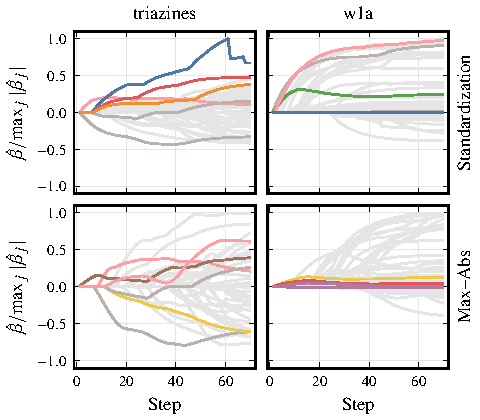
\includegraphics[]{plots/realdata_paths_small.pdf}
  \caption{%
    Lasso paths for \data{triazines}~\citep{king} and
    \data{w1a}~\citep{platt1998} using standardization and maximum absolute
    value normalization. (See \Cref{sec:data-summary} for details
    on these data sets and \Cref{fig:realdata-paths-full} in
    \Cref{sec:extended-real-data-paths} for an extended example.) For each data
    set we color the coefficients if they are among the first five to become
    non-zero under either normalization scheme.
  }
  \label{fig:realdata-paths}
\end{figure}

In spite of this relationship between normalization and regularization, there has so far
been no research on the topic. Instead, the choice of normalization is often motivated by
computational aspects or by being ``standard''. Because, although standardization is a
natural choice when the features are normally distributed, the choice is not as
straightforward for other types of data. In particular, there is no obvious strategy for
normalizing binary features (where the each observations takes either of two values) and no
previous research that have studied this problem before.
% Anecdotal suggestions include not normalizing at all or to normalize as you would if it
% were continuous data---the implications of either of these suggestions (or in deed any
% other), however, have yet to be investigated.

In this paper we begin to bridge this knowledge gap by studying normalization in the
context of three particular cases of \Cref{eq:general-objective}: the lasso, ridge, and
elastic net~\citep{zou2005}. The latter of these, the elastic net, is a generalization of
the previous two, and is represented by the following optimization problem:
%
\begin{equation}
  \label{eq:elastic-net}
  \operatorname*{minimize}_{\beta_0 \in \mathbb{R},\vec{\beta} \in \mathbb{R}^p} \frac{1}{2} \lVert \vec y - \beta_0 - \tilde{\mat{X}}\vec{\beta} \rVert^2_2  + \lambda_1 \lVert \vec\beta \rVert_1 + \frac{\lambda_2}{2}\lVert \vec \beta \rVert_2^2,
\end{equation}
%
where setting \(\lambda_1 = 0\) results in ridge regression and setting \(\lambda_2 = 0\) result in
the lasso.
% These methods are staples in the field of statistics and machine
% learning and are accompanied by a large body of theoretical work and applications for real
% data.

Our focus in this paper is on binary data and we will pay particular attention to the case
when binary features are imbalanced, that is, have relatively many ones or zeroes. In this
scenario, we will demonstrate that the choice of normalization directly influences the
regression coefficients and that this effect depends on the particular choice of
normalization and regularization.
